\documentclass[11pt, oneside]{article} 
\usepackage{geometry}
\geometry{letterpaper} 
\usepackage{graphicx}
	
\usepackage{amssymb}
\usepackage{amsmath}
\usepackage{parskip}
\usepackage{color}
\usepackage{hyperref}

\graphicspath{{/Users/telliott_admin/Dropbox/Tex/png/}}
% \begin{center} 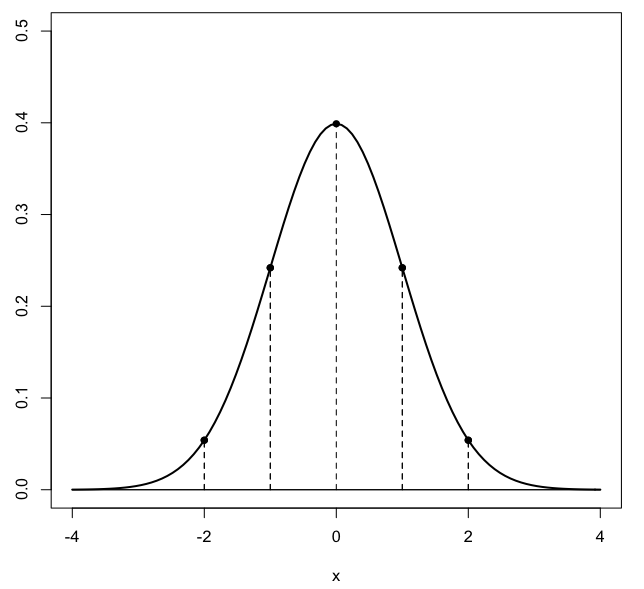
\includegraphics [scale=0.4] {gauss3.png} \end{center}

\title{Hyperbola}
\date{}

\begin{document}
\maketitle
\Large

\label{sec:Hyperbola_geometry}

Here is a hyperbola as shown in the wikipedia article on the subject.
\begin{center} 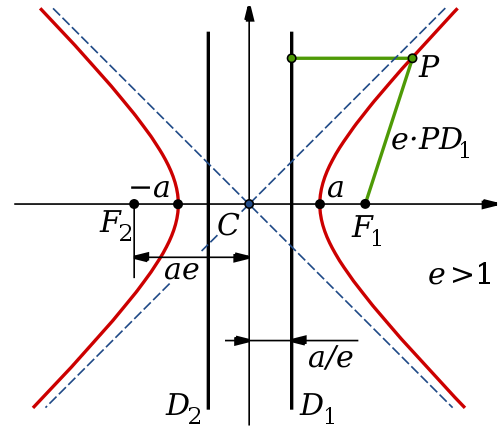
\includegraphics [scale=0.4] {hyper.png} \end{center}
Hyperbolas of this type (that open "east-west") have equations of the form
\[ \frac{x^2}{a^2} - \frac{y^2}{b^2} = 1 \]
Rearranging
\[ \frac{x^2}{a^2} = 1 + \frac{y^2}{b^2}\]
so the minimum value of $x$ occurs when $y=0$ and $x=a$.  

The \emph{conjugate} hyperbola of this one is
\[ \frac{x^2}{a^2} - \frac{y^2}{b^2} = -1 \]
or equivalently 
\[ -\frac{x^2}{a^2} + \frac{y^2}{b^2} = 1 \]
opens "north-south."  

And, although I will wait to deal with this complication, we have to mention another very common hyperbola
\[ xy = c \]
where it must be true that $x \ne 0$ and $y \ne 0$.

Another feature of hyperbolas is the asymptote, the straight line which is approached when $x,y >> a,b$.  In the case of the first example
\[ \frac{y^2}{b^2} = \frac{x^2}{a^2} - 1 \]
\[ y^2 = \frac{b^2}{a^2} x^2 - \frac{1}{a^2} \]
but for large $x$ and $y$ this approaches
\[ y^2 = \frac{b^2}{a^2} x^2 \]
\[ y = \pm \frac{b}{a} x \]
As the diagram suggests:
\begin{center} 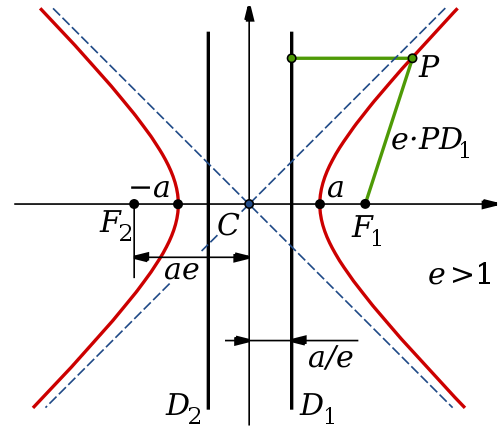
\includegraphics [scale=0.35] {hyper.png} \end{center}

The following diagram gives geometric meaning to the $b$ coefficient which really derives from the slope of the asymptotic line.  We go vertically up from $x=a$ to the asymptote and then go left to the $y-$axis, that intercept is $b$.

\begin{center} 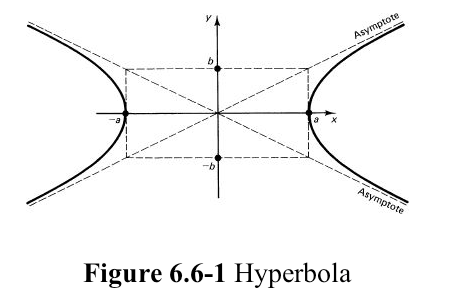
\includegraphics [scale=0.5] {hyperbola_box.png} \end{center}

\subsection*{geometry}
Kline gives the following string and pencil construction for the hyperbola.
\begin{center} 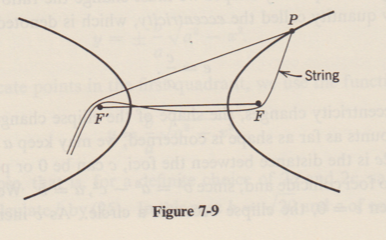
\includegraphics [scale=0.8] {Kline_7_9.png} \end{center}
Pick two foci $F$ and $F'$ and loop a long piece of string around them, holding it tight.  Then place the pencil at some point $P$ on a line between the two foci, at a fixed position in the upper loop.

Now let the string slowly slip up past $F'$ in both directions, increasing the length of $PF$ and $PF'$ by the same amount for each small slip.  What this amounts to is that the difference $PF - PF'$ is constant.

If we place the origin halfway between $F$ and $F'$ then
\begin{center} 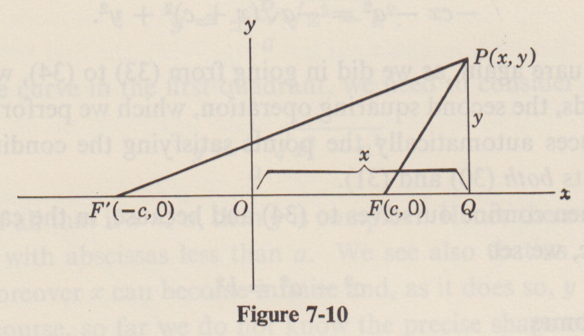
\includegraphics [scale=0.5] {Kline_7_10.png} \end{center}
\[ PF = \sqrt{(x - c)^2 + y^2} \]
\[ PF' = \sqrt{(x + c)^2 + y^2} \]
and the difference $PF' - PF$ is
\[ \sqrt{(x + c)^2 + y^2} - \sqrt{(x - c)^2 + y^2}  \]
and if the constant distance 
\[ PF' - PF = 2a \]
then
\[ \sqrt{((x + c)^2 + y^2} - \sqrt{(x - c)^2 + y^2} = 2a \]

Now we repeat the approach we took for the ellipse:
\[ \sqrt{((x + c)^2 + y^2} = 2a + \sqrt{(x - c)^2 + y^2} \]
Square
\[ (x + c)^2 + y^2 = 4a^2 + 4a\sqrt{(x + c)^2 + y^2} + (x - c)^2 + y^2 \]
Cancel $y^2$
\[ (x + c)^2 = 4a^2 + 4a\sqrt{(x + c)^2 + y^2} + (x - c)^2 \]
Since
\[ (x+c)^2 - (x - c)^2 = 4cx \]
we have
\[ 4cx = 4a^2 + 4a\sqrt{(x + c)^2 + y^2} \]
\[ cx - a^2 = a\sqrt{(x + c)^2 + y^2} \]
\[ c^2x^2 - 2ca^2x + a^4 = a^2(x + c)^2 + a^2y^2 \]
\[ c^2x^2 - 2ca^2x + a^4 = a^2x^2 + 2a^2cx + a^2c^2 + a^2y^2 \]
\[ (c^2 - a^2) x^2 - a^2y^2 = (c^2 - a^2) a^2 \]
Define $b^2$ slightly differently here
\[ b^2 = c^2 - a^2 \]
so
\[ b^2 x^2 - a^2y^2 = b^2 a^2 \]
\[ \frac{x^2}{a^2} - \frac{y^2}{b^2} = 1 \]
which looks familiar.

\end{document}  